%%%%%%%%%%%%%%%%%%%%%%%%%%%%
%% D A T A    M E M O R Y %%
%%%%%%%%%%%%%%%%%%%%%%%%%%%%

\subsection{Data Memory}
\label{subsec:data_memory}

The Data Memory block encapsulates the multi-bank memory used to store cache data. Each bank stores the data corresponding to a specific way across all cache sets.

Each memory bank is implemented as a pseudo-dual-port memory with a single memory access port that can be used for either a read or a write operation. Read requests are issued by the CPU-side cache logic, while write requests are generated from the R-channel of the external memory-side AXI4-Lite interface. The access type is selected according to the current cache operation.

When a read request is received, the corresponding set index is used to address each memory bank. On the following clock cycle, the Data Memory block provides the data stored in all ways of the selected set.

Both read and write operations have a latency of one clock cycle.

\begin{figure}[H]
	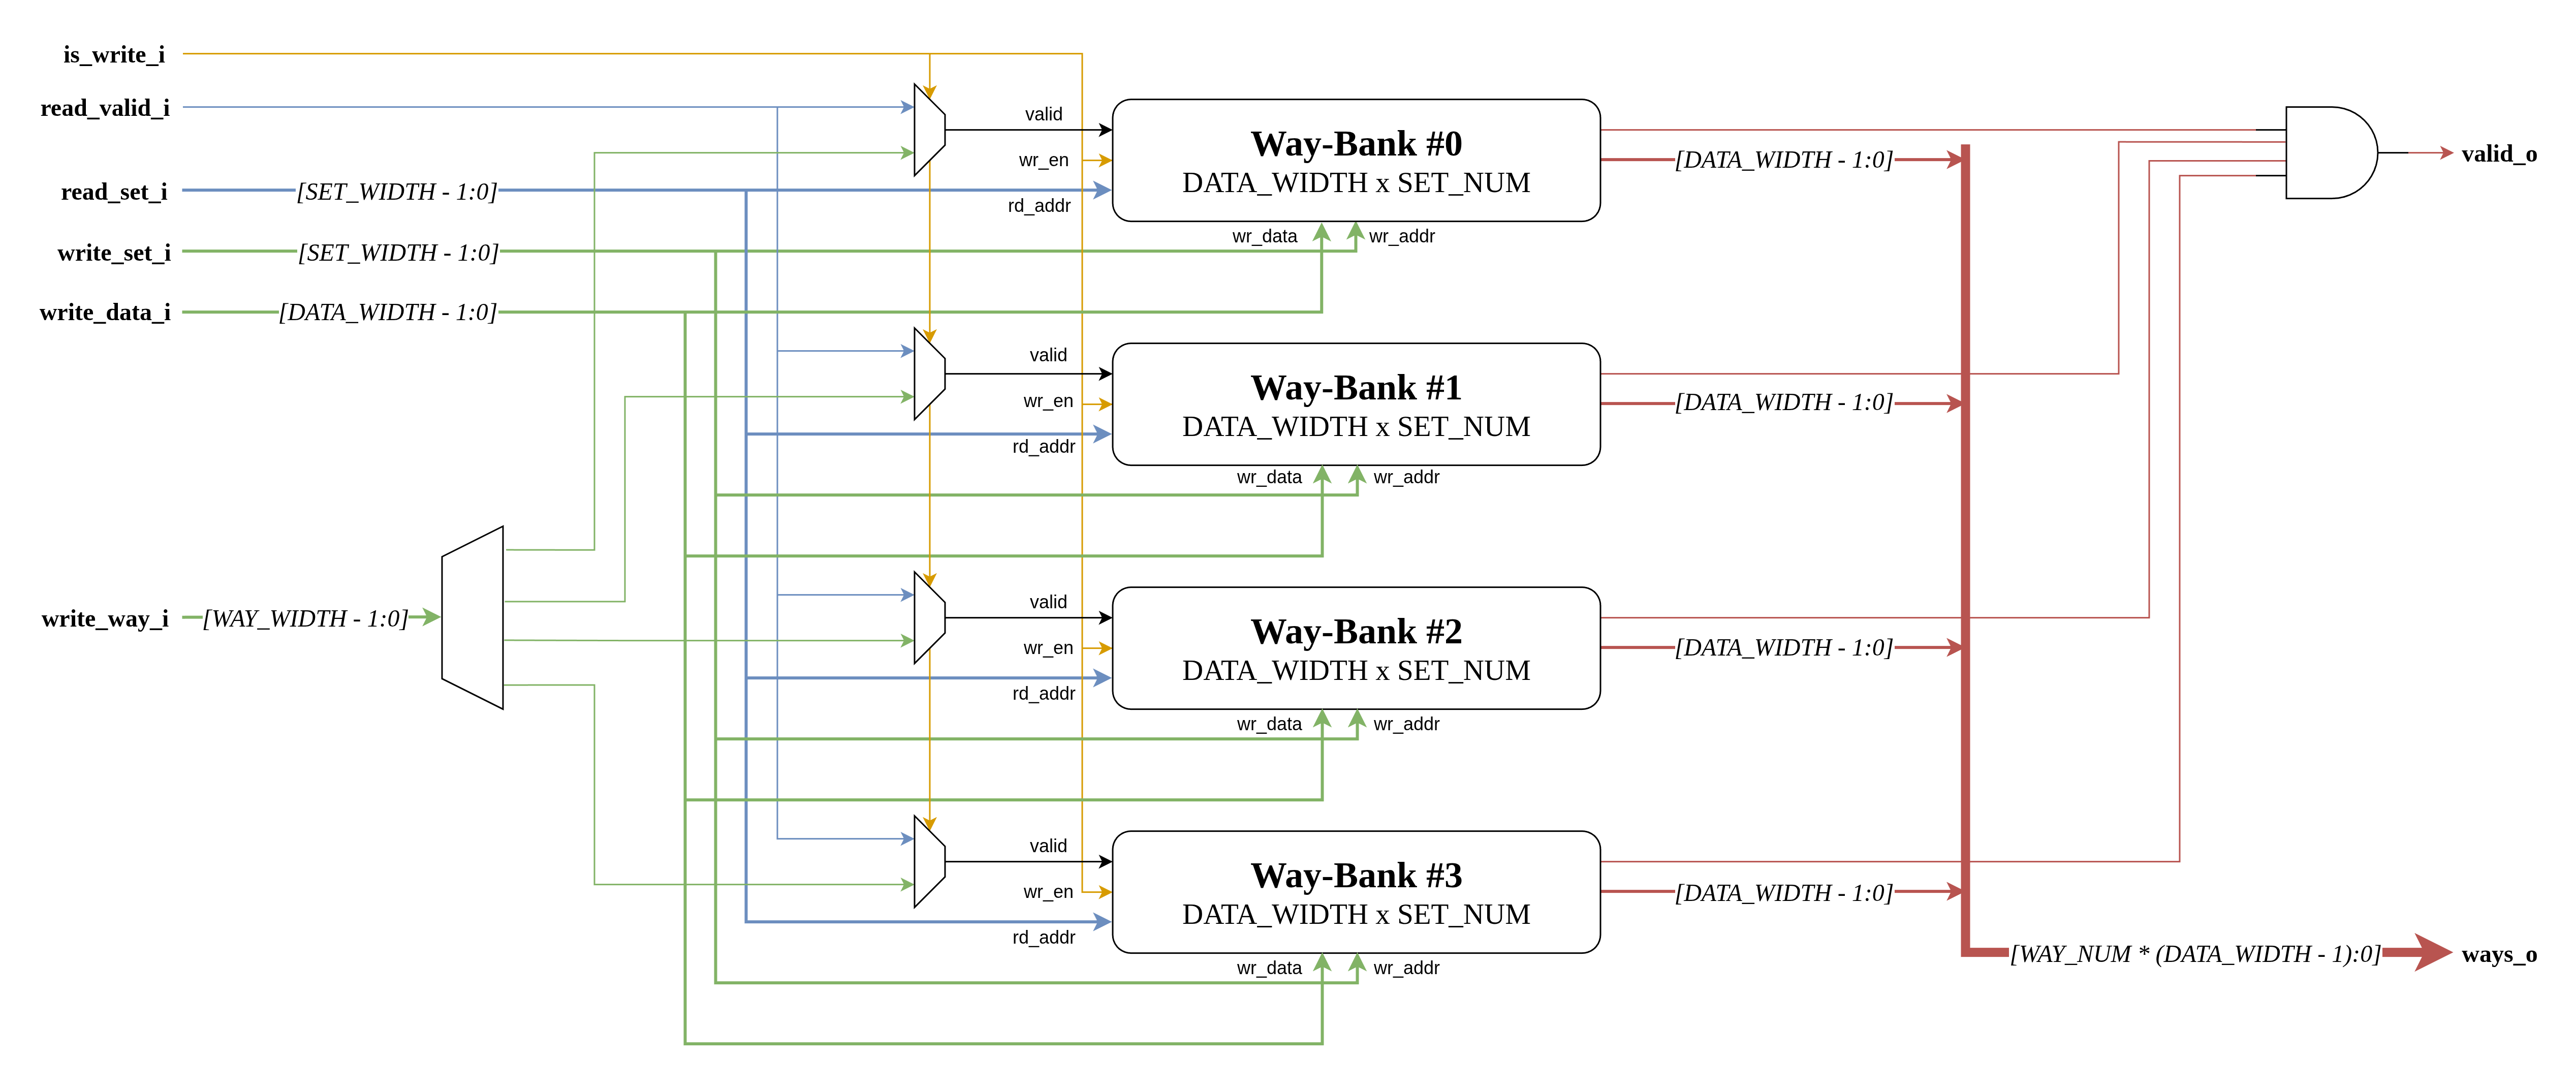
\includegraphics[width=16cm]{Data_Memory.png}
	\caption{Data Memory scheme (4-way cache)}
\end{figure}

\begin{table}[H]
	\centering
	\small
	\begin{tabularx}{\textwidth}{l c c X}
		\toprule
		\textbf{Parameter} & \textbf{Valid Range} & \textbf{Default} & \textbf{Description} \\
		\midrule
		
		\verb|DATA_WIDTH| &
		Positive integer &
		\verb|32| &
		Width of the data stored in each cache line. \\
		
		\verb|WAY_NUM| &
		Power of 2 &
		--- &
		Number of cache ways. \\
		
		\verb|SET_NUM| &
		Power of 2 &
		--- &
		Number of cache sets. \\
		
		\bottomrule
	\end{tabularx}
	\caption{Data Memory parameters}
	\label{tab:data_memory_parameters}
\end{table}

\begin{table}[htbp]
	\centering
	\label{tab:data_memory_ports}
	\small
	\begin{tabularx}{\textwidth}{l c c X}
		\toprule
		\textbf{Ports} & \textbf{Direction} & \textbf{Width} & \textbf{Description} \\
		\midrule
		\verb| read_valid_i | & Input & \verb| 1 | & Indicates a valid read request. \\
		\verb| read_set_i | & Input & \verb| SET_WIDTH | & Index of the cache set to be read. \\
		\verb| write_set_i | & Input & \verb| SET_WIDTH | & Index of the cache set to which the data is written. \\
		\verb| write_data_i | & Input & \verb| DATA_WIDTH | & Data to be written to the selected cache line. \\
		\verb| write_way_i | & Input & \verb| WAY_WIDTH | & Index of the way in which the input data is stored. \\
		\verb| valid_o | & Output & \verb| 1 | & Indicates that valid output data. \\
		\verb| ways_o | & Output & \verb| DATA_WIDTH * WAY_NUM | & Data stored in all ways of the requested cache set. \\
		\bottomrule
	\end{tabularx}
	\caption{Data Memory ports}
\end{table}